\documentclass[11pt]{article}
\usepackage{geometry,marginnote} % Pour passer au format A4
\geometry{hmargin=1cm, vmargin=1cm} % 

% Page et encodage
\usepackage[T1]{fontenc} % Use 8-bit encoding that has 256 glyphs
\usepackage[english,french]{babel} % Français et anglais
\usepackage[utf8]{inputenc} 

\usepackage{lmodern}
\setlength\parindent{0pt}

% Graphiques
\usepackage{graphicx,float,grffile}
\usepackage{pst-eucl, pst-plot,units} 

% Maths et divers
\usepackage{amsmath,amsfonts,amssymb,amsthm,verbatim}
\usepackage{multicol,enumitem,url,eurosym,gensymb}
\DeclareUnicodeCharacter{20AC}{\euro}

% Sections
\usepackage{sectsty} % Allows customizing section commands
\allsectionsfont{\centering \normalfont\scshape}

% Tête et pied de page

\usepackage{fancyhdr} 
\pagestyle{fancyplain} 

\fancyhead{} % No page header
\fancyfoot{}

\renewcommand{\headrulewidth}{0pt} % Remove header underlines
\renewcommand{\footrulewidth}{0pt} % Remove footer underlines

\newcommand{\horrule}[1]{\rule{\linewidth}{#1}} % Create horizontal rule command with 1 argument of height

%----------------------------------------------------------------------------------------
%   Début du document
%----------------------------------------------------------------------------------------

\begin{document}

\setlength{\columnseprule}{1pt}

\horrule{2px}
\section*{Chapitre 1 - Comprendre un exercice de mathématiques de $3^{ème}$ - \texttt{(T)}}
\horrule{2px}

L'objectif de ce chapitre est savoir communiquer en mathématiques pour avoir de bonnes notes. 

\section*{1 - J'ai un calcul à faire}

Je me rappelle des priorités de calcul de base. J'essaye de ne pas faire d'erreurs dès qu'un signe - apparait. J'essaye de ne pas me décomposer dès que je vois une fraction... \\

\textbf{J'utilise ma calculatrice. J'aurai toujours le droit à l'utiliser. Elle est personnelle et individuelle. Elle n'est pas juste utilisée pour obtenir le résultat. On peut aussi s'en servir pour trouver des résultats intermédiaires.}

\begin{align*}
8 +  2 \times 5 - (-4 + 2) \div 2 + 1 &= 8 + 10 - (-2) \div 2 + 1 \\
                                      &= 18 + 1  +1 \\
                                      &= 20
\end{align*}


\begin{align*}
\dfrac{1}{2} + \dfrac{3}{5} &= \dfrac{1 \times 5}{2 \times 5} + \dfrac{3 \times 2}{5 \times 2} \\
                            &= \dfrac{5}{10} + \dfrac{6}{10} \\
                            &= \dfrac{11}{10}
\end{align*}

\begin{center}\reversemarginpar\marginnote{$\Box \Box$}
\reversemarginpar\marginnote{$\Box \Box$}[0.3cm]
\reversemarginpar\marginnote{$\Box \Box$}[0.6cm]
\reversemarginpar\marginnote{$\Box \Box$}[0.9cm]
\fbox{\begin{minipage}{0.6\textwidth}{\bfseries 
    \begin{itemize}
    \item Il faut écrire des étapes.
    \item Il faut passer à la ligne à chaque calcul.
    \item (On aligne les fractions correctement.)    
    \item On aligne chaque signe égal.
    \item (On souligne le résultat.)
    \end{itemize}}
\end{minipage}}\end{center}

\textbf{Remarque} : \\
\textit{Attention, toutes les calculatrices ne donnent pas toujours les mêmes résultats} : $8 \div 2(2+2) =$ 16 (TI) ou 1 (Casio)

\begin{minipage}[t]{0.5\textwidth}
  \begin{figure}[H]
        \centering
        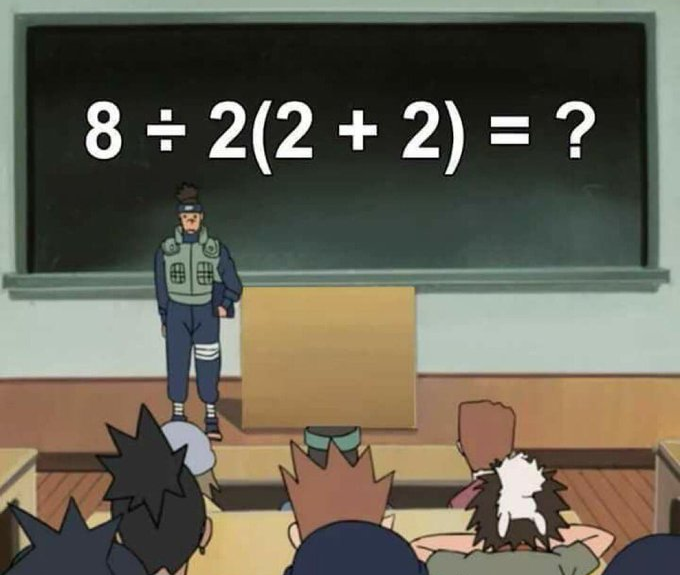
\includegraphics[width=0.7\linewidth]{3x1-calcul-algebrique-et-litteral/naruto.png}
  \end{figure}
\end{minipage}
\begin{minipage}[t]{0.5\textwidth}
  \begin{figure}[H]
        \centering
        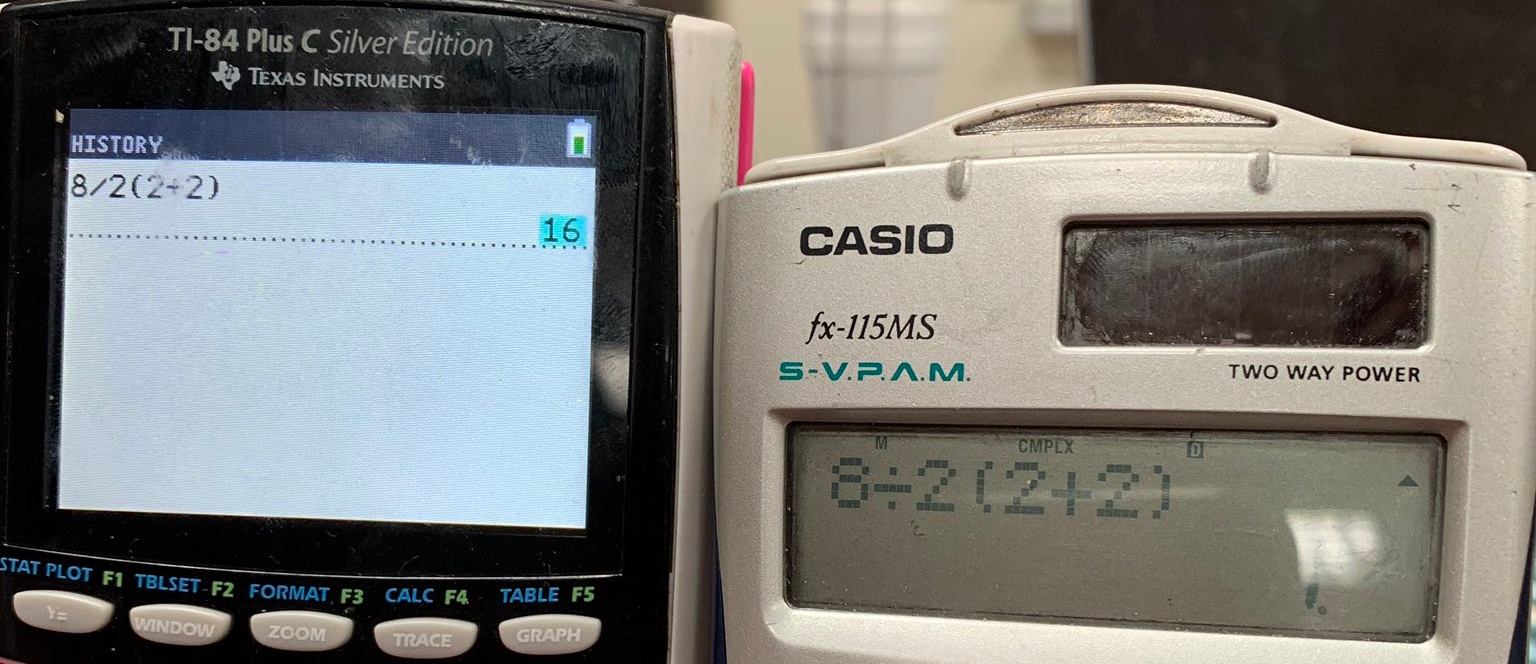
\includegraphics[width=\linewidth]{3x1-calcul-algebrique-et-litteral/calc.png}
  \end{figure}
... cela veut dire que le calcul est mal écrit ...
\end{minipage}

\newpage

\section*{2 - J'ai un problème}

Parfois les exercices de type problème ne donnent pas directement le ou les calculs à faire. Il parfois faire plusieurs calculs, il faut parfois créer une expression. On appelle cette compétence : \textbf{Modéliser}.\\

\subsection*{2 - J'ai un problème "simple"}

\textsc{\textbf{Exercice} : Pour la rentrée, j'achète une règle à 1,20€, trois crayons à papiers à 1,10€ l'unité et deux 4-couleurs à 2,50€.} \newline
\textsc{Je donne un billet de 10€, combien doit-on me rendre en caisse ?}\\

\begin{minipage}[t]{0.5\textwidth}
\textsc{\textbf{a. Correction avec une étape} :}\\

Calcul du prix à payer :
\begin{align*}
1,20 + 3 \times 1,10 + 2 \times 2,50 &= 1,20 + 3,30 + 5 \\
                                     &= 9,5
\end{align*}

Rendu : $10 - 9,5 = 0,5$

On doit me rendre 50 centimes.\\

\end{minipage}\begin{minipage}[t]{0.5\textwidth}
\textsc{\textbf{b. Correction sans étape} :}\\

Rendu :
\begin{align*}
10 - (1,20 + 3 \times 1,10 + 2 \times 2,50) &= 10 - 9,5 \\
                                            &= 0,5
\end{align*}

On doit me rendre 50 centimes. \\
\end{minipage}

On essaye de remarquer comment j’ai rédigé mes calculs. On appelle cette compétence \textbf{communiquer}. On parle de \textbf{convention d'écriture}.

\begin{center}
\reversemarginpar\marginnote{$\Box \Box$}
\reversemarginpar\marginnote{$\Box \Box$}[0.3cm]
\reversemarginpar\marginnote{$\Box \Box$}[0.6cm]
\fbox{\begin{minipage}{0.6\textwidth}{\bfseries 
    \begin{itemize}
    \item Il faut dire quels calculs on fait.
    \item Il faut créer des expressions à calculer. (Modéliser)
    \item Il faut rédiger les calcul avec les étapes.
    \item Il faut faire une phrase réponse.
    \end{itemize}}
\end{minipage}}
\end{center}


\subsection*{2 - J'ai un problème "compliqué"}

Parfois, les problèmes ne peux être résolu juste par un calcul. Il va falloir passer par une équation, un théorème... \\

\textsc{\textbf{Exercice} : Pour la rentrée, j'ai achète une règle à 1,20€, quatre crayons à papiers et trois 4-couleurs à 2,40€. J'ai payé 12€} \newline
\textsc{Quel est le prix d'un crayon de couleur ?}\\

On ne peut pas faire le calcul directement... Le but n'est pas juste de tâtonner... On doit passer par une méthode mathématique : une équation. Ces chapitres seront aussi l'occasion de faire des révisions. \\

\textsc{\textbf{Correction} :}\\

On pose $x$ le prix d'un crayon à papier.
\begin{align*}
& 1,20 + 4 \times x + 3 \times 2,40) = 12 \\
& 1,20 + 7,2 + 4x = 12 \\
& 8,4 + 4x = 12 \\
& 4x = 12 - 8,4\\
& 4x = 3,6
& x = 3,6 \div 4
& x = 0,9
\end{align*}

Un crayon à papier coûte 90 centimes.

\begin{center}
\fbox{\textbf{Il va falloir commencer à se comporter comme un mathématicien.}}
\end{center}

\end{document}
